% Created 2020-09-15 Tue 14:54
% Intended LaTeX compiler: pdflatex
\documentclass[9pt]{extarticle}
\usepackage[utf8]{inputenc}
\usepackage[T1]{fontenc}
\usepackage{chessboard}
\storechessboardstyle{4x4}{maxfield=d4}
\storechessboardstyle{4x1}{maxfield=a4}
\storechessboardstyle{4x2}{maxfield=b4}
\storechessboardstyle{1x4}{maxfield=d1}
\storechessboardstyle{2x4}{maxfield=d2}
\usepackage{tikz}
\usepackage{forest}
\usepackage{graphicx}
\usepackage{grffile}
\usepackage{longtable}
\usepackage{wrapfig}
\usepackage{rotating}
\usepackage[normalem]{ulem}
\usepackage{amsmath}
\usepackage{textcomp}
\usepackage{amssymb}
\usepackage{capt-of}
\usepackage[hidelinks]{hyperref}
% \usepackage{minted}
\usepackage[a4paper, total={6in, 9in}]{geometry}
% \setminted{breaklines, autogobble}
% \usemintedstyle{emacs}
\author{Nebhrajani A. V.}
\date{\today}
\title{\huge ZIO Select Answers}
\hypersetup{
 pdfauthor={Aditya V. Nebhrajani},
 pdftitle={IP OTBA Answers},
 pdfkeywords={},
 pdfsubject={},
 pdfcreator={Emacs 25.2.2 (Org mode 9.3.6)},
 pdflang={English}}
\begin{document}

\maketitle
% \tableofcontents

This document outlines my answers to some ZIO questions I found
interesting or instructive. The solutions are written the way I solved
them. In some cases, the solution is much better than the equivalent
given in answer keys, in others, the answer key does the job
better.

\section{2010}
\subsection{Org-Trees}

On first observation, the problem seems incredibly difficult to do
because of the sheer number of combinations one can achieve in large
org trees. The key insight, however, is that trees can (and should) be
seen recursively bottom-up, a technique in dynamic programming.

Consider the simple tree (direction of arrows is omitted where
hierarchies are obvious):
\begin{center}
  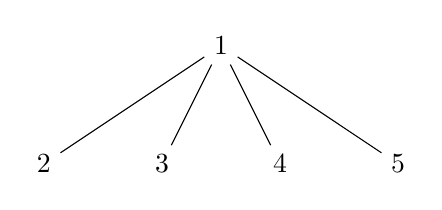
\begin{tikzpicture}
    \node {1} child {node {2}} child {node {3}} child {node {4}} child
    {node {5}};
  \end{tikzpicture}
\end{center}

In how many ways can we delete a leaf level node? Obviously,
only one way: just delete it. However, note that we always have the
option of \emph{not} deleting the node as well, giving us a total of 2
ways of dealing with leaves. Now, apply combinatorics. The total number of ways of deleting $1$ (or
below) will be the product of the ways of deleting its children, plus
one for its own deletion.

Therefore, writing number of ways of deletion into the tree:
\begin{center}
  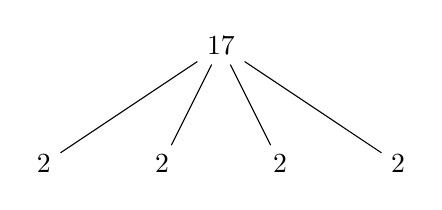
\begin{tikzpicture}
    \node {$17$} child {node {$2$}} child {node {$2$}} child {node {$2$}} child
    {node {$2$}};
  \end{tikzpicture}
\end{center}

And the problem is solved. Solving the first subproblem as an example,
\begin{center}
  \begin{forest}
    [1 [2 [5]] [3 [6 [10] [11]] [7 [12] [13] [14]]] [4 [8] [9]]]
  \end{forest}
\end{center}

Solving bottom-up:

\begin{center}
  \begin{forest}
    [691 [3 [2]] [46 [5 [2] [2]] [9 [2] [2] [2]]] [5 [2] [2]]]
  \end{forest}
\end{center}


\section{2011}
\subsection{n-Rooks Problem}
A famous problem in chess is the n-queens problem, or placing $N$
queens on an $N\times N$ chessboard such that none of them threaten
each other. Below is a solution for $N=4$.

\begin{center}
  \chessboard[style=4x4,setwhite={Qa2,Qb4, Qc1, Qd3},showmover=false]
  \hspace{1pt} \chessboard[style=4x4,setwhite={Ra3,Rb4, Rb2, Rc2},showmover=false]
\end{center}

The given problem can be thought of as an n-rooks problem, where no
two rooks may threaten each other. As you may have guessed, this is an
easier job than queens, since we don't have to worry about diagonal threats
anymore. It is therefore possible to view the given example as a
4$\times$4 chessboard, with some rooks threatening each other.

We are now left with calculating how to move these rooks so that they
don't threaten each other. It is sufficient to consider this one axis
at a time, in the following way. First consider threats only along the
$x$-axis, and draw a board by collapsing empty squares. Move a minimal
number of times to reduce this board to a $1\times N$ board, then
recompress. Repeat for the next axis. For the $x$-axis:

\begin{center}
  \chessboard[style=4x2,setwhite={Ra3,Ra4, Ra2, Rb2},showmover=false] \hspace{1pt}  \chessboard[style=4x1,setwhite={Ra3,Ra4, Ra2, Ra1},showmover=false]
\end{center}

Moving Rb2 down and recompressing, we get the desired board. This took
one move. (Recompressing is a visual aid and does not count as a
move.) Therefore, $M_x = 1$. Now, along the $y$-axis:


\begin{center}
  \chessboard[style=2x4,setwhite={Ra2,Rb2, Rb1, Rc2},showmover=false] \hspace{1pt} \chessboard[style=2x4,setwhite={Ra2,Rb2, Rc1, Rd2},showmover=false] \hspace{1pt}  \chessboard[style=1x4,setwhite={Ra1,Rb1, Rc1, Rd1},showmover=false]
\end{center}

To compress down, we must either move Rc2 to d2 and Rb1 to c1 (two
moves) or move Rb1 to d1 (also two moves). So, $M_y = 2$. $$\sum M =
M_x + M_y = 1 + 2 = 3$$

Solve all subparts similarly. Be careful while doing compressions:
choose a \emph{minimum} number of moves to compress. This will always
mean moving a piece to the closest empty row or column, and not one
further away. This can be done by directly moving the piece or by
swapping in a chain: both of which will require the same number of
moves, as shown above.


\end{document}